\subsection{Reichweite von $\alpha$-Strahlung}
Die Messdaten zu der Reichweite der $\alpha$-Strahlung sind in den Tabellen \ref{tab:reichweite15} und \ref{tab:reichweite20} notiert.
Die effektive Länge $x$ berechnet sich nach Gleichung \eqref{eqn:x}.
Als Normaldruck $p_{\text{0}}$ wird $p_{\text{0}}=\SI{1013}{mbar}$ \cite{1} verwendet.
%\begin{align*}
%  x = x_{\text{0}} \frac{p }{p_{\text{0}}}
%\end{align*}
\begin{table}[h!]
  \centering
  \caption{Messdaten zur Reichweite der $\alpha$-Strahlung bei dem Abstand $x_{\text{0}}=\SI{15e-3}{m}$}
  \label{tab:reichweite15}
  \begin{tabular}{c c c c c c}
    \toprule
      $p/mbar$ & x/$10^{-3}m$  &  counts &  channel &  N/$\SI{120}{s}$ & E/$MeV$   \\
      \midrule
         0     &      -   &   250   &   1198   &    117202   &  4,000  \\
        50     &   0,740  &   257   &   1168   &    116734   &  3,899  \\
       100     &   1,481  &   266   &   1137   &    115567   &  3,796  \\
       150     &   2,221  &   262   &   1117   &    113857   &  3,730  \\
       200     &   2,962  &   281   &   1092   &    113411   &  3,646  \\
       250     &   3,702  &   274   &   1062   &    111891   &  3,546  \\
       300     &   4,442  &   293   &   1030   &    111018   &  3,439  \\
       350     &   5,183  &   306   &   995    &    108357   &  3,322  \\
       400     &   5,923  &   318   &   977    &    107255   &  3,262  \\
       450     &   6,663  &   319   &   946    &    106426   &  3,159  \\
       500     &   7,404  &   326   &   927    &    103909   &  3,095  \\
       550     &   8,144  &   340   &   904    &    102456   &  3,018  \\
       600     &   8,885  &   341   &   875    &     99858   &  2,921  \\
       650     &   9,625  &   342   &   840    &     96111   &  2,805  \\
       700     &  10,365  &   360   &   811    &     92348   &  2,708  \\
       750     &  10,922  &   373   &   778    &     87965   &  2,598  \\
       800     &  11,846  &   379   &   761    &     83617   &  2,541  \\
       850     &  12,586  &   398   &   721    &     75036   &  2,407  \\
       900     &  13,327  &   394   &   750    &     84841   &  2,504  \\
       950     &  14,067  &   419   &   695    &     59568   &  2,321  \\
      1000     &  14,808  &   421   &   667    &     50722   &  2,227  \\

    \bottomrule
  \end{tabular}
\end{table}

%\end{landscape}
%\end{document}

\begin{figure}[h!]
  \centering
  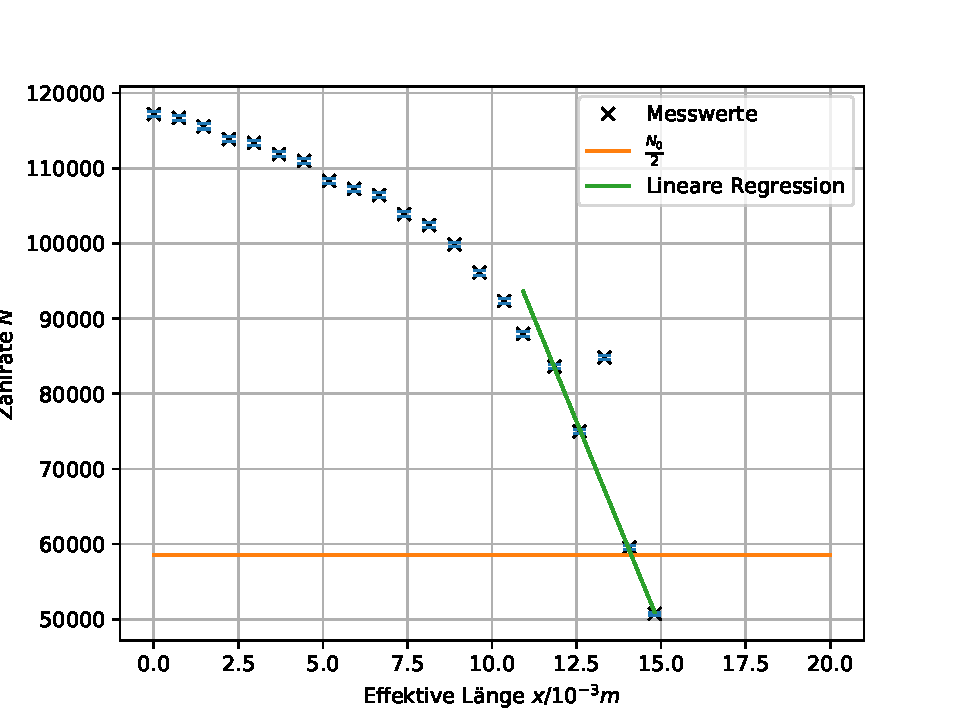
\includegraphics[width=\textwidth]{reichweite15.pdf}
  \caption{Zählrate $N$ gegen die effektive Länge $x$ für den Abstand $x_{\text{0}}=\SI{15e-3}{m}$}
  \label{fig:reichweite15}
\end{figure}
\begin{table}[h!]
  \centering
  \caption{Messdaten zur Reichweite der $\alpha$-Strahlung bei dem Abstand $x_{\text{0}}=\SI{20e-3}{m}$}
  \label{tab:reichweite20}
  \begin{tabular}{c c c c c c}
    \toprule
      $p/mbar$ & x/$10^{-3}m$ & counts &  channel &  N/$\SI{120}{s}$  &  E/$MeV$ \\
      \midrule
         0     &   -      &  230    &  1231    &    85500   &  4,000  \\
        50     &   0,987  &  188    &  1201    &    85385   &  3,903  \\
       100     &   1,974  &  190    &  1158    &    85004   &  3,763  \\
       150     &   2,962  &  198    &  1126    &    84394   &  3,659  \\
       200     &   3,949  &  207    &  1096    &    82912   &  3,561  \\
       250     &   4,936  &  210    &  1057    &    80758   &  3,435  \\
       300     &   5,923  &  219    &  1020    &    80509   &  3,314  \\
       350     &   6,910  &  218    &   986    &    79362   &  3,204  \\
       400     &   7,897  &  238    &   956    &    77502   &  3,106  \\
       450     &   8,885  &  244    &   916    &    75228   &  2,976  \\
       500     &   9,872  &  256    &   889    &    72848   &  2,889  \\
       550     &  10,859  &  259    &   844    &    69387   &  2,742  \\
       600     &  11,846  &  268    &   810    &    66006   &  2,632  \\
       650     &  12,833  &  270    &   766    &    59688   &  2,489  \\
       700     &  13,820  &  279    &   728    &    53991   &  2,366  \\
       750     &  14,806  &  299    &   691    &    43968   &  2,245  \\
       800     &  15,795  &  285    &   672    &    34330   &  2,184  \\
       850     &  16,782  &  248    &   668    &    23138   &  2,171  \\
       900     &  17,769  &  186    &   672    &    13991   &  2,184  \\
       950     &  18,756  &  104    &   665    &     7618   &  2,161  \\
      1000     &  19,743  &   49    &   662    &     3320   &  2,151  \\


    \bottomrule
  \end{tabular}
\end{table}

%\end{landscape}
%\end{document}

\begin{figure}[h!]
  \centering
  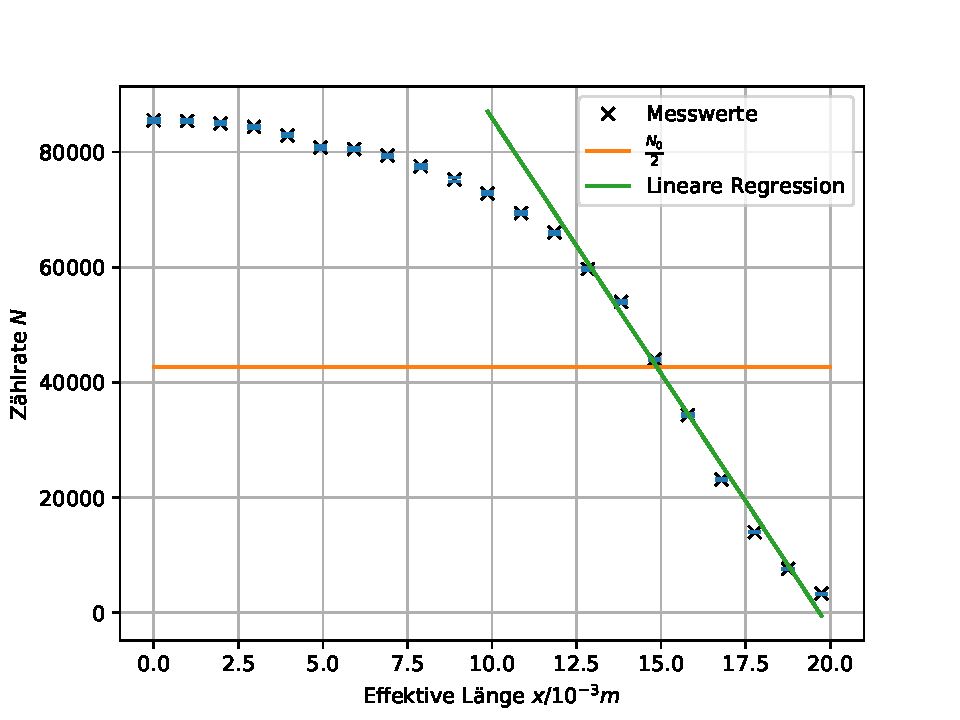
\includegraphics[width=\textwidth]{reichweite20.pdf}
  \caption{Zählrate $N$ gegen die effektive Länge $x$ für den Abstand $x_{\text{0}}=\SI{15e-3}{m}$}
  \label{fig:reichweite20}
\end{figure}
Die Zählraten $N$ werden gegen die effektiven Längen $x$ aufgetragen (Abb. \ref{fig:reichweite15}, Abb. \ref{fig:reichweite20}).
Außerdem wird die Hälfte der jeweiligen der maximalen Zählrate $N_{\text{max}}$ markiert.
Weiterhin wird durch den linearen Anteil der geplotteten Messwerte eine lineare Regression der Form:
\begin{align*}
  y=mx+b
\end{align*}
mittels Python gelegt.
Der Schnittpunkt der beiden Geraden berechnet sich entsprechend über
\begin{align}
  \frac{N_{\text{max}}}{2}=mx+b \Leftrightarrow x= \frac{1}{m} \left( \frac{N_{\text{max}}}{2}-b \right)
\label{eqn:schnittpunkt}
\end{align}
Die Parameter zu beiden linearen Regressionen lauten:
\begin{align*}
  m_{\text{15}}=& \SI{-11161.81319114 \pm 194.581e3}{\frac{1}{m}}\\
  b_{\text{15}}=& \SI{213533.63549628 \pm 2560.195}{}\\
  m_{\text{20}}=& \SI{-8865.00722469 \pm 508.736e3}{\frac{1}{m}}\\
  b_{\text{20}}=& \SI{174533.89481311 \pm 8596.284}{}.\\
\end{align*}
Nach Gleichung \eqref{eqn:schnittpunkt} ergeben sich nun die Schnittpunkte:
\begin{align*}
x_{\text{15}}=& \SI{13.881 \pm 0.242e-3}{m} \\
x_{\text{20}}=& \SI{14.866 \pm 1.550e-3}{m}.\\
\end{align*}
Die beiden Fehler werden mithilfe der Gauß'schen Fehlerfortpflanzung berechnet:
\begin{align*}
  \Delta x_{\text{15}}  &=&  \sqrt{ \left(-\frac{1}{m_{\text{15}}^2} \left( \frac{N_{\text{15}}}{2} - b_{\text{15}} \right) \right)^2 \Delta m_{\text{15}}^2 + \left(-\frac{1}{m_{\text{15}}} \right)^2 \Delta b_{\text{15}}^2}  &=& \SI{0.242e-3}{\frac{1}{m}}\\
  \Delta x_{\text{20}}  &=& \sqrt{ \left( -\frac{1}{m_{\text{20}}^2} \left( \frac{N_{\text{20}}}{2} - b_{\text{20}} \right) \right)^2 \Delta m_{\text{20}}^2 + \left(-\frac{1}{m_{\text{20}}} \right)^2 \Delta b_{\text{20}}^2}  &=& \SI{1.550e-3}{\frac{1}{m}}\\
\end{align*}
Diese Schnittpunkte entsprechen den Reichweiten der $\alpha$-Strahlung.
Zur Energiebestimmung ist der Channel-Wert nötig.
Die maximale Energie $E=\SI{4}{MeV}$ ist linear mit dem Channel-Wert beim minimalen Druck verknüpft.
Entsprechend werden mit dieser Relation die Energiewerte berechnet.
Die Energien $E$ sind in den Abbildungen \ref{fig:e15} und \ref{fig:e20} gegen die effektiven Längen $x$ aufgetragen.
\begin{figure}[h!]
  \centering
  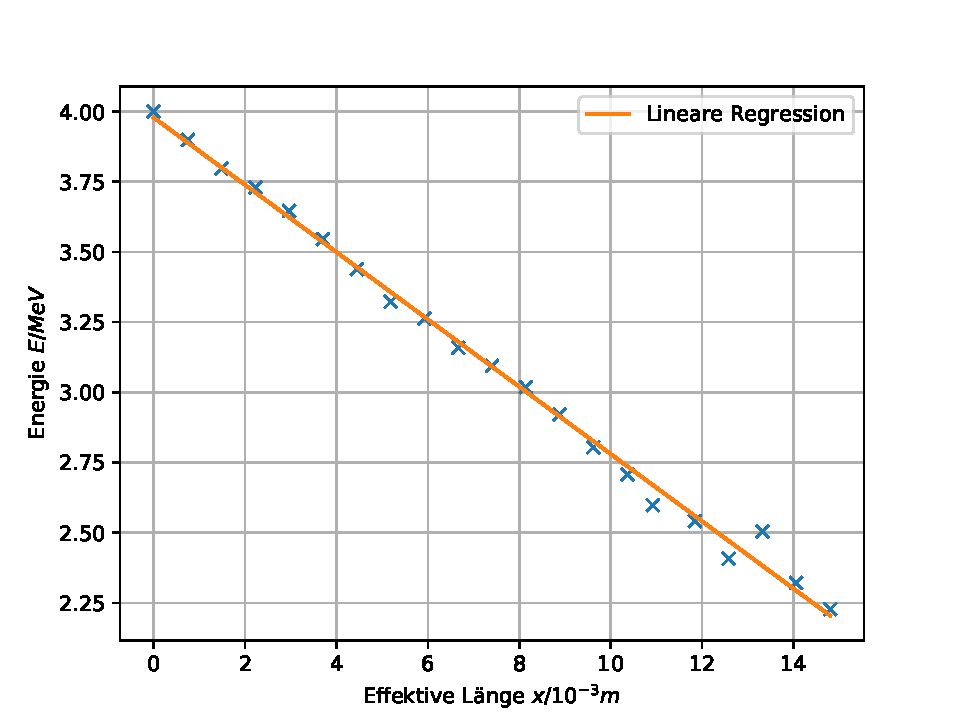
\includegraphics[width=\textwidth]{e15.pdf}
  \caption{Energie $E$ gegen die effektive Länge $x$ für den Abstand $x_{\text{0}}=\SI{15e-3}{m}$}
  \label{fig:e15}
\end{figure}
\begin{figure}[h!]
  \centering
  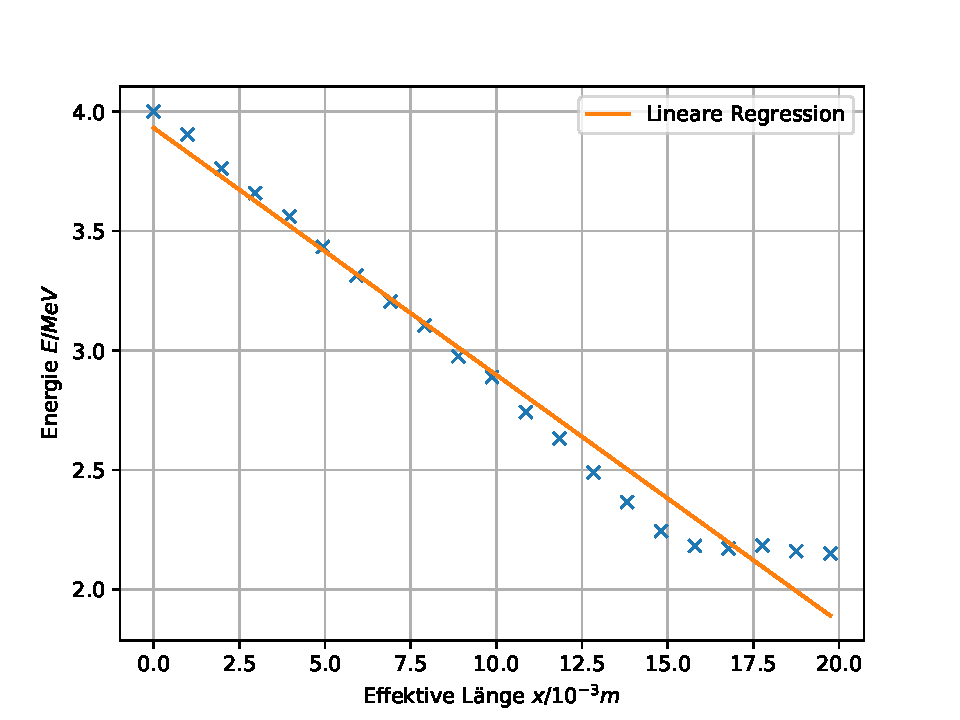
\includegraphics[width=\textwidth]{e20.pdf}
  \caption{Energie $E$ gegen die effektive Länge $x$ für den Abstand $x_{\text{0}}=\SI{15e-3}{m}$}
  \label{fig:e20}
\end{figure}
Die Parameter der linearen Regressionen der Form $y=nx+c$ lauten:
\begin{align*}
  \frac{dE_{\text{15}}}{dx}   &=& n_{\text{15}} &=& \SI{-119.78612 \pm 1.957012041}{\frac{MeV}{m}}\\
                              & & c_{\text{15}} &=& \SI{ 3.97839549 \pm 0.016916861850}{MeV}\\
  \frac{dE_{\text{20}}}{dx}   &=& n_{\text{20}} &=& \SI{-103.33675 \pm 3.752994338}{\frac{MeV}{m}}\\
                              & & c_{\text{20}} &=& \SI{ 3.93129148 \pm 0.043310806270}{MeV}.\\
\end{align*}
Die negativen Steigungen der linearen Regressionen entsprechen den Energieverlusten $\frac{dE}{dx}$.

\FloatBarrier

\subsection{Statistik des radioaktiven Zerfalls}
\begin{table}[h!]
  \centering
  \caption{Messdaten zur Statistik des $\alpha$-Zerfalls}
  \label{tab:stat}
  \begin{tabular}{c c c c}
    \toprule
      N & N & N & N \\
    \midrule
      9421    &   8888    &    9237   &   9599\\
      9281    &   9010    &    9217   &   8933\\
      8710    &   9052    &    9031   &   9103\\
      9063    &   8610    &    8894   &   9261\\
      9262    &   9707    &    8861   &   8790\\
      9573    &   9781    &    9063   &   9387\\
      9297    &   9734    &    8965   &   9064\\
      9502    &   9560    &    9306   &   9583\\
      8839    &   9267    &    9516   &   9528\\
      9411    &   9166    &    9464   &   8976\\
      9039    &   9568    &    9392   &   9002\\
      9442    &   9505    &    8964   &   9452\\
      9371    &   9836    &    9196   &   9040\\
      9533    &   9255    &    9438   &   8800\\
      9016    &   9090    &    9648   &   9077\\
      9549    &   9768    &    9256   &   9427\\
      9196    &   9016    &    9565   &   8863\\
      8931    &   9158    &    9588   &   8849\\
      8965    &   9300    &    9263   &   9432\\
      9403    &   9567    &    9740   &   8892\\
      8861    &   9169    &    9522   &   8894\\
      9508    &   9399    &    9482   &   9217\\
      9545    &   9015    &    9653   &   9355\\
      9432    &   8701    &    9562   &   9209\\
      9465    &   9601    &    8925   &   9330\\


    \bottomrule
  \end{tabular}
\end{table}

Die Messdaten zur Überprüfung der Statistik des radioaktiven Zerfalls sind in Tabelle \ref{tab:stat} notiert.
Die Zählraten sind in Abbildung \ref{fig:stat} als Histogramm mit Python aufgetragen.
Der Mittelwert $\mu$, die korrigierte Standardabweichung $\sigma$ und die Standardabweichung des Mittelwertes $\sigma_{\mu}$ der Messdaten $x_{\text{m}}$ berechnen sich bei einer Messdatenanzahl $M$ durch:
\begin{align*}
  \mu           &=&                           &=& \frac{1}{M} \sum_{m=1}^{M} x_{m}                                   &=& \SI{9261.49}{} \\
  \sigma        &=&                           &=& \sqrt{\frac{1}{M-1} \sum_{m=1}^{M} |x_{m}-\mu|^2}                  &=& \SI{287.39}{}\\
  \sigma_{\mu}  &=&  \frac{\sigma}{\sqrt{M}}  &=& \frac{1}{\sqrt{M}} \sqrt{\frac{1}{M} \sum_{m=1}^{M} |x_{m}-\mu|^2} &=& \SI{28.739}{}.\\
\end{align*}
Damit werden eine beispielhafte Gaußverteilung und eine beispielhafte Poissonverteilung in das Histogramm gelegt.
\begin{figure}[h!]
  \centering
  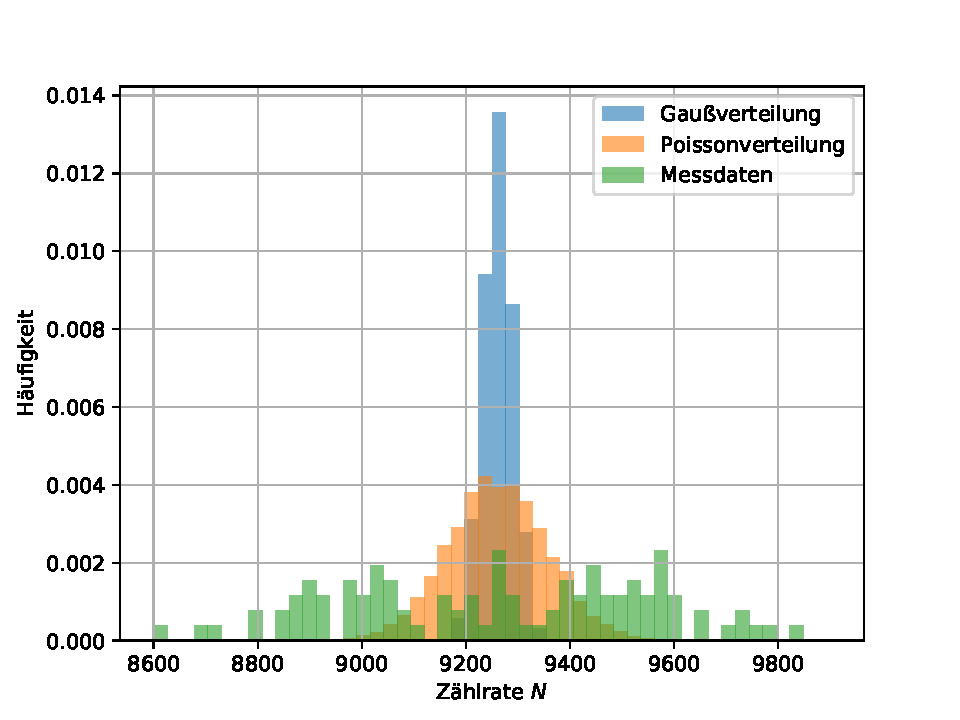
\includegraphics[width=\textwidth]{stat.pdf}
  \caption{Zählrate $N$ als Histogramm ihrer Häufigkeit}
  \label{fig:stat}
\end{figure}

\FloatBarrier
